%!TEX root = ../../deco_star.tex

\begin{table*}
    \tiny
    \centering
%     \resizebox{0.9\textwidth}{!}{
    
%     \begin{tabu} to \textwidth {
%         |[1pt middleGray] X[10,l] 
%         >{\columncolor[gray]{0.9}}X[1,c]
%         >{\columncolor[gray]{0.9}}X[1,c]
%         X[1,c]
%         X[1,c]
%         X[1,c]
%         >{\columncolor[gray]{0.9}}X[1,c]
%         >{\columncolor[gray]{0.9}}X[1,c]
%         X[1,c]
%         X[1,c]
%         X[1,c]
%         >{\columncolor[gray]{0.9}}X[1,c]
%         >{\columncolor[gray]{0.9}}X[1,c]
%         >{\columncolor[gray]{0.9}}X[1,c]
%         X[1,c]
%         X[1,c]
%         >{\columncolor[gray]{0.9}}X[1,c]
%         >{\columncolor[gray]{0.9}}X[1,c]
%         |[1pt middleGray]
%         }
    
%     % \begin{tabu}{ |[1pt middleGray] l g g l l l g g l l l g g g l l g g|[1pt middleGray]}
    
%         \taburulecolor{middleGray}\hline
%         \tableHeaderStyle
    
%          & 
%         \multicolumn{2}{g}{INIT.} & 
%         \multicolumn{3}{g}{EXEMPLARS} &
%         \multicolumn{2}{g}{PARAM.} & 
%         \multicolumn{3}{g}{HANDLING} & 
%         \multicolumn{3}{g}{FILLING} & 
%         \multicolumn{2}{g}{GUIDING} & 
%         \multicolumn{2}{g|[1pt middleGray]}{PLACE.}
%         \\
    
%         & 
%         \sidy{Configuration} & \sidy{Initialization} & 
%         \sidy{Image} & \sidy{Arrangement} & \sidy{Element} &
%         \sidy{Visual Output } & \sidy{System} &
%         \sidy{Visualization} & \sidy{Image} & \sidy{Sketch} &
%         \sidy{Shapes} & \sidy{Masking} & \sidy{Curve} &
%         \sidy{Brushing} & \sidy{Directions} &
%         \sidy{Element} & \sidy{Drag \& Drop}
%         \\



% % --------------------------------------------------------------------------------
% % Distribution and Repetition
% % --------------------------------------------------------------------------------
%     \taburulecolor{middleGray}\hline
%     \multicolumn{18}{|[1pt middleGray]l|[1pt middleGray]}{\textit{\uppercase{Distribution and Repetition}}} \\
%     \taburulecolor{middleGray}\hline

%     % Stochastic Pattern
%     % --------------------------------------------------------------------------------
%     \multicolumn{18}{|[1pt middleGray]l|[1pt middleGray]}{\textit{Stochastic}} \\

%     \citeauthor*{galerne_2012_gne}~\cite{galerne_2012_gne} &
%     % INIT:
%     % Config & Task Init & 
%     & & 
%     % EXEMP:
%     % Image
%     % Element arrangement
%     % Element
%     $\times$ & & &
%     % PARAM:
%     % Visual output
%     % System/Generation
%     $\times$ & &
%     % CONTR:
%     % Custom visual UI
%     % Image-based
%     % Sketch-based
%     $\times$ & &  &
%     % FILL:
%     % Shapes
%     % Masking
%     % Curve/Strokes to fill
%     $\times$ & &  &
%     % GUIDE:
%     % Painting/Strokes to follow
%     % Directions
%     & &
%     % PLACE:
%     % Element Placement
%     % Element Drag&Drop
%     & 
%     \\

%     \citeauthor*{gilet_2012_mkn}~\cite{gilet_2012_mkn} &
%     % INIT:
%     % Config & Task Init & 
%     & $\times$ & 
%     % EXEMP:
%     % Image
%     % Element arrangement
%     % Element
%     $\times$ & & &
%     % PARAM:
%     % Visual output
%     % System/Generation
%     $\times$ & &
%     % CONTR:
%     % Custom visual UI
%     % Image-based
%     % Sketch-based
%     & $\times$ &  &
%     % FILL:
%     % Shapes
%     % Masking
%     % Curve/Strokes to fill
%     $\times$ & &  &
%     % GUIDE:
%     % Painting/Strokes to follow
%     % Directions
%     & &
%     % PLACE:
%     % Element Placement
%     % Element Drag&Drop
%     & 
%     \\
        
%     \citeauthor*{gilet_2014_lrn}~\cite{gilet_2014_lrn} &
%     % INIT:
%     % Config & Task Init & 
%     & & 
%     % EXEMP:
%     % Image
%     % Element arrangement
%     % Element
%     $\times$ & & &
%     % PARAM:
%     % Visual output
%     % System/Generation
%     $\times$ & $\times$ &
%     % CONTR:
%     % Custom visual UI
%     % Image-based
%     % Sketch-based
%     & $\times$ &  &
%     % FILL:
%     % Shapes
%     % Masking
%     % Curve/Strokes to fill
%     $\times$ & &  &
%     % GUIDE:
%     % Painting/Strokes to follow
%     % Directions
%     & &
%     % PLACE:
%     % Element Placement
%     % Element Drag&Drop
%     & 
%     \\

%     \citeauthor*{pavie_2016_pts}~\cite{pavie_2016_pts} &
%     % INIT:
%     % Config & Task Init & 
%     & & 
%     % EXEMP:
%     % Image
%     % Element arrangement
%     % Element
%     & & $\times$ &
%     % PARAM:
%     % Visual output
%     % System/Generation
%     $\times$ & $\times$ &
%     % CONTR:
%     % Custom visual UI
%     % Image-based
%     % Sketch-based
%     & $\times$ &  &
%     % FILL:
%     % Shapes
%     % Masking
%     % Curve/Strokes to fill
%     $\times$ & &  &
%     % GUIDE:
%     % Painting/Strokes to follow
%     % Directions
%     & &
%     % PLACE:
%     % Element Placement
%     % Element Drag&Drop
%     & 
%     \\


%     \citeauthor*{guingo_2017_btm}~\cite{guingo_2017_btm} &
%     % INIT:
%     % Config & Task Init & 
%     & & 
%     % EXEMP:
%     % Image
%     % Element arrangement
%     % Element
%     $\times$ & & & 
%     % PARAM:
%     % Visual output
%     % System/Generation
%     $\times$ & $\times$ &
%     % CONTR:
%     % Custom visual UI
%     % Image-based
%     % Sketch-based
%     & $\times$ &  &
%     % FILL:
%     % Shapes
%     % Masking
%     % Curve/Strokes to fill
%     $\times$ & &  &
%     % GUIDE:
%     % Painting/Strokes to follow
%     % Directions
%     & &
%     % PLACE:
%     % Element Placement
%     % Element Drag&Drop
%     & 
%     \\
    
%     \citeauthor*{kang_2017_fpt}~\cite{kang_2017_fpt} &
%     % INIT:
%     % Config & Task Init & 
%     & & 
%     % EXEMP:
%     % Image
%     % Element arrangement
%     % Element
%     $\times$ & & &
%     % PARAM:
%     % Visual output
%     % System/Generation
%     $\times$ & &
%     % CONTR:
%     % Custom visual UI
%     % Image-based
%     % Sketch-based
%     & $\times$ &  &
%     % FILL:
%     % Shapes
%     % Masking
%     % Curve/Strokes to fill
%     $\times$ & &  &
%     % GUIDE:
%     % Painting/Strokes to follow
%     % Directions
%     & &
%     % PLACE:
%     % Element Placement
%     % Element Drag&Drop
%     & 
%     \\
    
%     \citeauthor*{gilet_2010_ias}~\cite{gilet_2010_ias} &
%     % INIT:
%     % Config & Task Init & 
%     & $\times$ & 
%     % EXEMP:
%     % Image
%     % Element arrangement
%     % Element
%     $\times$ & & &
%     % PARAM:
%     % Visual output
%     % System/Generation
%     $\times$ & &
%     % CONTR:
%     % Custom visual UI
%     % Image-based
%     % Sketch-based
%     & & $\times$ &
%     % FILL:
%     % Shapes
%     % Masking
%     % Curve/Strokes to fill
%     $\times$ & &  &
%     % GUIDE:
%     % Painting/Strokes to follow
%     % Directions
%     & &
%     % PLACE:
%     % Element Placement
%     % Element Drag&Drop
%     & 
%     \\


%     % Regular to Irregular Pattern
%     % --------------------------------------------------------------------------------
%     \multicolumn{18}{|[1pt middleGray]l|[1pt middleGray]}{\textit{Regular to Irregular Pattern}} \\

%     % Example-Based
%         \citeauthor*{lefebvre_2000_ass}~\cite{lefebvre_2000_ass} &
%         % INIT:
%         % Config & Task Init & 
%         & $\times$ & 
%         % EXEMP:
%         % Image
%         % Element arrangement
%         % Element
%         $\times$ & & &
%         % PARAM:
%         % Visual output
%         % System/Generation
%         $\times$ & &
%         % CONTR:
%         % Custom visual UI
%         % Image-based
%         % Sketch-based
%         & $\times$ &  &
%         % FILL:
%         % Shapes
%         % Masking
%         % Curve/Strokes to fill
%         $\times$ & &  &
%         % GUIDE:
%         % Painting/Strokes to follow
%         % Directions
%         & &
%         % PLACE:
%         % Element Placement
%         % Element Drag&Drop
%         & 
%         \\

%         \citeauthor*{gilet_2012_map}~\cite{gilet_2012_map} &
%         % INIT:
%         % Config & Task Init & 
%         & & 
%         % EXEMP:
%         % Image
%         % Element arrangement
%         % Element
%         & $\times$ & $\times$ &
%         % PARAM:
%         % Visual output
%         % System/Generation
%         $\times$ & &
%         % CONTR:
%         % Custom visual UI
%         % Image-based
%         % Sketch-based
%         & &  &
%         % FILL:
%         % Shapes
%         % Masking
%         % Curve/Strokes to fill
%         $\times$ & &  &
%         % GUIDE:
%         % Painting/Strokes to follow
%         % Directions
%         & &
%         % PLACE:
%         % Element Placement
%         % Element Drag&Drop
%         & 
%         \\



%         \citeauthor*{bourque_2004_ptm}~\cite{bourque_2004_ptm} &
%         % INIT:
%         % Config & Task Init & 
%         $\times$ & $\times$ & 
%         % EXEMP:
%         % Image
%         % Element arrangement
%         % Element
%         $\times$ & & &
%         % PARAM:
%         % Visual output
%         % System/Generation
%         $\times$ & &
%         % CONTR:
%         % Custom visual UI
%         % Image-based
%         % Sketch-based
%         & &  &
%         % FILL:
%         % Shapes
%         % Masking
%         % Curve/Strokes to fill
%         $\times$ & &  &
%         % GUIDE:
%         % Painting/Strokes to follow
%         % Directions
%         & &
%         % PLACE:
%         % Element Placement
%         % Element Drag&Drop
%         & 
%         \\

%         \citeauthor*{gieseke_2014_ipr}~\cite{gieseke_2014_ipr} &
%         % INIT:
%         % Config & Task Init & 
%         $\times$ & $\times$ & 
%         % EXEMP:
%         % Image
%         % Element arrangement
%         % Element
%         $\times$ & & &
%         % PARAM:
%         % Visual output
%         % System/Generation
%         $\times$ & $\times$ &
%         % CONTR:
%         % Custom visual UI
%         % Image-based
%         % Sketch-based
%         & &  &
%         % FILL:
%         % Shapes
%         % Masking
%         % Curve/Strokes to fill
%         $\times$ & &  &
%         % GUIDE:
%         % Painting/Strokes to follow
%         % Directions
%         & &
%         % PLACE:
%         % Element Placement
%         % Element Drag&Drop
%         & 
%         \\

%         % Reference
%         \citeauthor*{hu_2019_anf}~\cite{hu_2019_anf} & 
%         % Config & Task Init & 
%         $\times$ & $\times$ & 
%         % Image & Element arrangement & Element &
%         $\times$ &  &  &
%         % Visual output  & System/Generation &
%         $\times$ &  & 
%         % Custom visual UI & Image-based  & Sketch-based &
%         &  &  &
%         % Shapes & Masking & Curve/Strokes to fill &
%         $\times$ &  &  &
%         % Painting/Strokes to follow & Directions  &
%         &  & 
%         % Element Placement & Element Drag&Drop
%         & 
%         \\


%         % Reference
%         \citeauthor*{guehl_2020_stu}~\cite{guehl_2020_stu} & 
%         % Config & Task Init & 
%             & $\times$ & 
%         % Image & Element arrangement & Element &
%         $\times$ &  &  &
%         % Visual output  & System/Generation &
%         $\times$ & $\times$ & 
%         % Custom visual UI & Image-based  & Sketch-based &
%         $\times$ & &  &
%         % Shapes & Masking & Curve/Strokes to fill &
%         $\times$ &  &  &
%         % Painting/Strokes to follow & Directions  &
%         &  & 
%         % Element Placement & Element Drag&Drop
%             & 
%         \\


%         % Data-Driven
%             % Reference
%             \citeauthor*{bian_2018_tpd}~\cite{bian_2018_tpd} & 
%             % Config & Task Init & 
%                 &  & 
%             % Image & Element arrangement & Element &
%             $\times$ &  &  &
%             % Visual output  & System/Generation &
%             &  & 
%             % Custom visual UI & Image-based  & Sketch-based &
%             $\times$ &  & $\times$ &
%             % Shapes & Masking & Curve/Strokes to fill &
%             $\times$  &  &  &
%             % Painting/Strokes to follow & Directions  &
%             &  & 
%             % Element Placement & Element Drag&Drop
%                 & 
%             \\
    
%             % Reference
%             \citeauthor*{li_2019_aqp}~\cite{li_2019_aqp} & 
%             % Config & Task Init & 
%                 & $\times$ & 
%             % Image & Element arrangement & Element &
%             &  &  &
%             % Visual output  & System/Generation &
%             $\times$ & $\times$ & 
%             % Custom visual UI & Image-based  & Sketch-based &
%                 &  &  &
%             % Shapes & Masking & Curve/Strokes to fill &
%             $\times$ &  &  &
%             % Painting/Strokes to follow & Directions  &
%             &  & 
%             % Element Placement & Element Drag&Drop
%                 & 
%             \\

%             \citeauthor*{tu_2020_cct}~\cite{tu_2020_cct} & 
%             % Config & Task Init & 
%             &  & 
%             % Image & Element arrangement & Element &
%             & $\times$ &  &
%             % Visual output  & System/Generation &
%             &  $\times$ & 
%             % Custom visual UI & Image-based  & Sketch-based &
%             $\times$ &  & $\times$ &
%             % Shapes & Masking & Curve/Strokes to fill &
%             $\times$ &  &  &
%             % Painting/Strokes to follow & Directions  &
%             &  & 
%             % Element Placement & Element Drag&Drop
%             $\times$ & $\times$
%             \\

%             \citeauthor*{zehnder_2016_dso}~\cite{zehnder_2016_dso} &
%             % INIT:
%             % Config & Task Init & 
%              &  & 
%             % EXEMP:
%             % Image
%             % Element arrangement
%             % Element
%              & & $\times$ &
%             % PARAM:
%             % Visual output
%             % System/Generation
%              & $\times$ & 
%             % CONTR:
%             % Custom visual UI
%             % Image-based
%             % Sketch-based
%             $\times$ & &  &
%             % FILL:
%             % Shapes
%             % Masking
%             % Curve/Strokes to fill
%             $\times$ & &  &
%             % GUIDE:
%             % Painting/Strokes to follow
%             % Directions
%             & &
%             % PLACE:
%             % Element Placement
%             % Element Drag&Drop
%             $\times$ & $\times$
%             \\

%             \citeauthor*{chen_2016_sof}~\cite{chen_2016_sof} & 
%             % INIT:
%             % Config & Task Init & 
%             & $\times$ & 
%             % EXEMP:
%             % Image
%             % Element arrangement
%             % Element
%             & & &
%             % PARAM:
%             % Visual output
%             % System/Generation
%             $\times$ & &
%             % CONTR:
%             % Custom visual UI
%             % Image-based
%             % Sketch-based
%             & &  &
%             % FILL:
%             % Shapes
%             % Masking
%             % Curve/Strokes to fill
%             $\times$ & $\times$ &  &
%             % GUIDE:
%             % Painting/Strokes to follow
%             % Directions
%             & $\times$ &
%             % PLACE:
%             % Element Placement
%             % Element Drag&Drop
%             & 
%             \\

%     % Rule-based and Design-Specific Pattern
%     % --------------------------------------------------------------------------------
%     \multicolumn{18}{|[1pt middleGray]l|[1pt middleGray]}{\textit{Rule- and Design-Specific Pattern}} \\


%     \citeauthor*{wong_1998_cgf}~\cite{wong_1998_cgf} & 
%         % INIT:
%         % Config & Task Init & 
%         $\times$ & & 
%         % EXEMP:
%         % Image
%         % Element arrangement
%         % Element
%         & & &
%         % PARAM:
%         % Visual output
%         % System/Generation
%         $\times$ & &
%         % CONTR:
%         % Custom visual UI
%         % Image-based
%         % Sketch-based
%         & &  &
%         % FILL:
%         % Shapes
%         % Masking
%         % Curve/Strokes to fill
%         $\times$ & &  &
%         % GUIDE:
%         % Painting/Strokes to follow
%         % Directions
%         & &
%         % PLACE:
%         % Element Placement
%         % Element Drag&Drop
%         & 
%         \\
%         \citeauthor*{santoni_2016_ggp}~\cite{santoni_2016_ggp} & 
%         % INIT:
%         % Config & Task Init & 
%         & & 
%         % EXEMP:
%         % Image
%         % Element arrangement
%         % Element
%         & & &
%         % PARAM:
%         % Visual output
%         % System/Generation
%         $\times$ & $\times$&
%         % CONTR:
%         % Custom visual UI
%         % Image-based
%         % Sketch-based
%         & &  $\times$&
%         % FILL:
%         % Shapes
%         % Masking
%         % Curve/Strokes to fill
%         $\times$ & $\times$ &  &
%         % GUIDE:
%         % Painting/Strokes to follow
%         % Directions
%         & &
%         % PLACE:
%         % Element Placement
%         % Element Drag&Drop
%         & 
%         \\

%         \citeauthor*{loi_2017_pae}~\cite{loi_2017_pae} & 
%         % INIT:
%         % Config & Task Init & 
%         $\times$ & & 
%         % EXEMP:
%         % Image
%         % Element arrangement
%         % Element
%         & & &
%         % PARAM:
%         % Visual output
%         % System/Generation
%         $\times$ & &
%         % CONTR:
%         % Custom visual UI
%         % Image-based
%         % Sketch-based
%         & &  &
%         % FILL:
%         % Shapes
%         % Masking
%         % Curve/Strokes to fill
%         $\times$ & &  &
%         % GUIDE:
%         % Painting/Strokes to follow
%         % Directions
%         & &
%         % PLACE:
%         % Element Placement
%         % Element Drag&Drop
%         & 
%         \\


%         % Probabilistic Interference
%         \citeauthor*{talton_2011_mpm}~\cite{talton_2011_mpm} & 
%         % INIT:
%         % Config & Task Init & 
%         $\times$ & & 
%         % EXEMP:
%         % Image
%         % Element arrangement
%         % Element
%         & & &
%         % PARAM:
%         % Visual output
%         % System/Generation
%         $\times$ & &
%         % CONTR:
%         % Custom visual UI
%         % Image-based
%         % Sketch-based
%         & $\times$ &  &
%         % FILL:
%         % Shapes
%         % Masking
%         % Curve/Strokes to fill
%         $\times$ & $\times$ &  &
%         % GUIDE:
%         % Painting/Strokes to follow
%         % Directions
%         & &
%         % PLACE:
%         % Element Placement
%         % Element Drag&Drop
%         & 
%         \\
%         \citeauthor*{ritchie_2015_cpm}~\cite{ritchie_2015_cpm} & 
%         % INIT:
%         % Config & Task Init & 
%         $\times$ & & 
%         % EXEMP:
%         % Image
%         % Element arrangement
%         % Element
%         & & &
%         % PARAM:
%         % Visual output
%         % System/Generation
%         $\times$ & &
%         % CONTR:
%         % Custom visual UI
%         % Image-based
%         % Sketch-based
%         & $\times$ &  &
%         % FILL:
%         % Shapes
%         % Masking
%         % Curve/Strokes to fill
%         $\times$ & $\times$ &  &
%         % GUIDE:
%         % Painting/Strokes to follow
%         % Directions
%         & &
%         % PLACE:
%         % Element Placement
%         % Element Drag&Drop
%         & 
%         \\

%         % Vector Field
%         \citeauthor*{yuanyuan_2011_gso}~\cite{yuanyuan_2011_gso} & 
%         % Config & Task Init & 
%         $\times$ & & 
%         % Image & Element arrangement & Element &
%          &  &  &
%         % Visual output  & System/Generation &
%         $\times$ &  & 
%         % Custom visual UI & Image-based  & Sketch-based &
%          &  &  &
%         % Shapes & Masking & Curve/Strokes to fill &
%         $\times$ &  &  &
%         % Painting/Strokes to follow & Directions  &
%          & $\times$ & 
%         % Element Placement & Element Drag&Drop
%          & 
%         \\

%         % Example-Based Control
%         \citeauthor*{stava_2010_ipm}~\cite{stava_2010_ipm} &
%         % INIT:
%         % Config & Task Init & 
%         & $\times$ & 
%         % EXEMP:
%         % Image
%         % Element arrangement
%         % Element
%         & $\times$ & &
%         % PARAM:
%         % Visual output
%         % System/Generation
%         $\times$ & $\times$ &
%         % CONTR:
%         % Custom visual UI
%         % Image-based
%         % Sketch-based
%         & &  &
%         % FILL:
%         % Shapes
%         % Masking
%         % Curve/Strokes to fill
%         $\times$ & &  &
%         % GUIDE:
%         % Painting/Strokes to follow
%         % Directions
%         & &
%         % PLACE:
%         % Element Placement
%         % Element Drag&Drop
%         & 
%         \\

%         \citeauthor*{talton_2012_ldp}~\cite{talton_2012_ldp} &
%         % INIT:
%         % Config & Task Init & 
%         & $\times$ & 
%         % EXEMP:
%         % Image
%         % Element arrangement
%         % Element
%         & $\times$ & &
%         % PARAM:
%         % Visual output
%         % System/Generation
%         $\times$ & $\times$ &
%         % CONTR:
%         % Custom visual UI
%         % Image-based
%         % Sketch-based
%         & &  &
%         % FILL:
%         % Shapes
%         % Masking
%         % Curve/Strokes to fill
%         $\times$ & &  &
%         % GUIDE:
%         % Painting/Strokes to follow
%         % Directions
%         & &
%         % PLACE:
%         % Element Placement
%         % Element Drag&Drop
%         & 
%         \\



%     % Element Arrangements
%     % --------------------------------------------------------------------------------
%     \multicolumn{18}{|[1pt middleGray]l|[1pt middleGray]}{\textit{Element Arrangements}} \\

%         % Example-Based Control
%         \citeauthor*{barla_2006_spa}~\cite{barla_2006_spa} &
%         % INIT:
%         % Config & Task Init & 
%         & $\times$ & 
%         % EXEMP:
%         % Image
%         % Element arrangement
%         % Element
%         & $\times$ & &
%         % PARAM:
%         % Visual output
%         % System/Generation
%         $\times$ & &
%         % CONTR:
%         % Custom visual UI
%         % Image-based
%         % Sketch-based
%         & &  &
%         % FILL:
%         % Shapes
%         % Masking
%         % Curve/Strokes to fill
%         & &  &
%         % GUIDE:
%         % Painting/Strokes to follow
%         % Directions
%         & &
%         % PLACE:
%         % Element Placement
%         % Element Drag&Drop
%         & 
%         \\

%         \citeauthor*{hurtut_2009_ags}~\cite{hurtut_2009_ags} &
%         % INIT:
%         % Config & Task Init & 
%         & & 
%         % EXEMP:
%         % Image
%         % Element arrangement
%         % Element
%         & $\times$ & &
%         % PARAM:
%         % Visual output
%         % System/Generation
%         & &
%         % CONTR:
%         % Custom visual UI
%         % Image-based
%         % Sketch-based
%         & $\times$ &  &
%         % FILL:
%         % Shapes
%         % Masking
%         % Curve/Strokes to fill
%         $\times$ & &  &
%         % GUIDE:
%         % Painting/Strokes to follow
%         % Directions
%         & &
%         % PLACE:
%         % Element Placement
%         % Element Drag&Drop
%         & 
%         \\

%         \citeauthor*{ijiri_2008_aeb}~\cite{ijiri_2008_aeb} &
%         % Config & Task Init & 
%         & & 
%         % Image
%         % Element arrangement
%         % Element
%         & $\times$ &  &
%         % Visual output
%         % System/Generation
%         $\times$ & $\times$ & 
%         % Custom visual UI
%         % Image-based
%         % Sketch-based
%         &  &  &
%         % Shapes
%         % Masking
%         % Curve/Strokes to fill
%         $\times$ & $\times$ &  &
%         % Painting/Strokes to follow
%         % Directions
%         $\times$ & $\times$ & 
%         % Element Placement
%         % Element Drag&Drop
%         & 
%         \\

%         \citeauthor*{ma_2011_det}~\cite{ma_2011_det} &
%         % INIT:
%         % Config & Task Init & 
%          & $\times$ & 
%         % EXEMP:
%         % Image
%         % Element arrangement
%         % Element
%          & $\times$ & &
%         % PARAM:
%         % Visual output
%         % System/Generation
%         $\times$  & $\times$ &
%         % CONTR:
%         % Custom visual UI
%         % Image-based
%         % Sketch-based
%          & &  &
%         % FILL:
%         % Shapes
%         % Masking
%         % Curve/Strokes to fill
%         $\times$ & &  &
%         % GUIDE:
%         % Painting/Strokes to follow
%         % Directions
%          & $\times$ & 
%         % PLACE:
%         % Element Placement
%         % Element Drag&Drop
%          & $\times$
%         \\

%         % Reference
%         \citeauthor*{almeraj_2013_pgt}~\cite{almeraj_2013_pgt} & 
%         % Config & Task Init & 
%             &  & 
%         % Image & Element arrangement & Element &
%         & $\times$ &  &
%         % Visual output  & System/Generation &
%         &  & 
%         % Custom visual UI & Image-based  & Sketch-based &
%             &  &  &
%         % Shapes & Masking & Curve/Strokes to fill &
%         $\times$ &  &  &
%         % Painting/Strokes to follow & Directions  &
%         &  & 
%         % Element Placement & Element Drag&Drop
%             & 
%         \\
        
        
%         \citeauthor*{landes_2013_asm}~\cite{landes_2013_asm} & 
%         % Config & Task Init & 
%             &  & 
%         % Image & Element arrangement & Element &
%         & $\times$ &  &
%         % Visual output  & System/Generation &
%         $\times$ & $\times$ & 
%         % Custom visual UI & Image-based  & Sketch-based &
%             & $\times$ &  &
%         % Shapes & Masking & Curve/Strokes to fill &
%         $\times$ &  &  &
%         % Painting/Strokes to follow & Directions  &
%         &  & 
%         % Element Placement & Element Drag&Drop
%             & 
%         \\

%         % Vector Fields
%                 % Reference
%                 \citeauthor*{saputra_2017_ffo}~\cite{saputra_2017_ffo} & 
%                 % Config & Task Init & 
%                     & $\times$ & 
%                 % Image & Element arrangement & Element &
%                     &  & $\times$ &
%                 % Visual output  & System/Generation &
%                     & & 
%                 % Custom visual UI & Image-based  & Sketch-based &
%                     &  & $\times$ &
%                 % Shapes & Masking & Curve/Strokes to fill &
%                 $\times$ & $\times$ &  &
%                 % Painting/Strokes to follow & Directions  &
%                     & $\times$ & 
%                 % Element Placement & Element Drag&Drop
%                 & 
%                 \\
%                 % Reference
%                 \citeauthor*{saputra_2018_rde}~\cite{saputra_2018_rde} & 
%                 % Config & Task Init & 
%                     & $\times$  & 
%                 % Image & Element arrangement & Element &
%                 &  & $\times$  &
%                 % Visual output  & System/Generation &
%                 &  & 
%                 % Custom visual UI & Image-based  & Sketch-based &
%                     &  &  &
%                 % Shapes & Masking & Curve/Strokes to fill &
%                 $\times$ &  &  &
%                 % Painting/Strokes to follow & Directions  &
%                 &  & 
%                 % Element Placement & Element Drag&Drop
%                     & 
%                 \\

%         % Data-Driven


% % --------------------------------------------------------------------------------
% % Frames and Hierarchies
% % --------------------------------------------------------------------------------
% \taburulecolor{middleGray}\hline
% \multicolumn{18}{|[1pt middleGray]l|[1pt middleGray]}{\textit{\uppercase{Frames and Hierarchies}}} \\
% \taburulecolor{middleGray}\hline

%             % Reference
%             \citeauthor*{anderson_2008_udt}~\cite{anderson_2008_udt} &
%             % INIT:
%             % Config & Task Init & 
%                 & & 
%             % EXEMP:
%             % Image
%             % Element arrangement
%             % Element
%                 & & $\times$ &
%             % PARAM:
%             % Visual output
%             % System/Generation
%             $\times$ & $\times$&
%             % CONTR:
%             % Custom visual UI
%             % Image-based
%             % Sketch-based
%                 & &  &
%             % FILL:
%             % Shapes
%             % Masking
%             % Curve/Strokes to fill
%             &$\times$& $\times$ &
%             % GUIDE:
%             % Painting/Strokes to follow
%             % Directions
%             & &
%             % PLACE:
%             % Element Placement
%             % Element Drag&Drop
%             $\times$ & 
%             \\

                        
%             \citeauthor*{benes_2011_gpm}~\cite{benes_2011_gpm} & 
%             % INIT:
%             % Config & Task Init & 
%             $\times$ & & 
%             % EXEMP:
%             % Image
%             % Element arrangement
%             % Element
%             & & &
%             % PARAM:
%             % Visual output
%             % System/Generation
%             $\times$ & &
%             % CONTR:
%             % Custom visual UI
%             % Image-based
%             % Sketch-based
%             $\times$ & &  &
%             % FILL:
%             % Shapes
%             % Masking
%             % Curve/Strokes to fill
%             $\times$ & $\times$ &  &
%             % GUIDE:
%             % Painting/Strokes to follow
%             % Directions
%             & &
%             % PLACE:
%             % Element Placement
%             % Element Drag&Drop
%             & 
%             \\


%             % Reference
%             \citeauthor*{gieseke_2017_ooo}~\cite{gieseke_2017_ooo} & 
%             % Config & Task Init & 
%             $\times$ & $\times$ & 
%             % Image & Element arrangement & Element &
%             &  &  &
%             % Visual output  & System/Generation &
%             $\times$ &  & 
%             % Custom visual UI & Image-based  & Sketch-based &
%             & $\times$ & $\times$ &
%             % Shapes & Masking & Curve/Strokes to fill &
%             $\times$ & $\times$ & $\times$ &
%             % Painting/Strokes to follow & Directions  &
%             & $\times$ & 
%             % Element Placement & Element Drag&Drop
%             $\times$ & $\times$
%             \\

%         % Data-Driven
%         \citeauthor*{lu_2014_dds}~\cite{lu_2014_dds} &
%         % INIT:
%         % Config & Task Init & 
%          & $\times$ & 
%         % EXEMP:
%         % Image
%         % Element arrangement
%         % Element
%          & & $\times$ &
%         % PARAM:
%         % Visual output
%         % System/Generation
%         $\times$ & &
%         % CONTR:
%         % Custom visual UI
%         % Image-based
%         % Sketch-based
%          & & $\times$ &
%         % FILL:
%         % Shapes
%         % Masking
%         % Curve/Strokes to fill
%          & & $\times$ &
%         % GUIDE:
%         % Painting/Strokes to follow
%         % Directions
%          & &
%         % PLACE:
%         % Element Placement
%         % Element Drag&Drop
%          & 
%         \\
    
    
%         \citeauthor*{zhou_2014_tsv}~\cite{zhou_2014_tsv} &
%         % INIT:
%         % Config & Task Init & 
%          & $\times$ & 
%         % EXEMP:
%         % Image
%         % Element arrangement
%         % Element
%          & & $\times$ &
%         % PARAM:
%         % Visual output
%         % System/Generation
%         $\times$ & $\times$ &
%         % CONTR:
%         % Custom visual UI
%         % Image-based
%         % Sketch-based
%          & &  &
%         % FILL:
%         % Shapes
%         % Masking
%         % Curve/Strokes to fill
%         $\times$ & & $\times$ &
%         % GUIDE:
%         % Painting/Strokes to follow
%         % Directions
%          & &
%         % PLACE:
%         % Element Placement
%         % Element Drag&Drop
%          & 
%         \\
    
    

% % --------------------------------------------------------------------------------
% % Curves, Lines and Brushing
% % --------------------------------------------------------------------------------
% \taburulecolor{middleGray}\hline
% \multicolumn{18}{|[1pt middleGray]l|[1pt middleGray]}{\textit{\uppercase{Curves, Lines and Brushing}}} \\
% \taburulecolor{middleGray}\hline


%         % Reference
%         \citeauthor*{yu_2012_ans}~\cite{yu_2012_ans} &
%         % INIT:
%         % Config & Task Init & 
%          & & 
%         % EXEMP:
%         % Image
%         % Element arrangement
%         % Element
%          & & &
%         % PARAM:
%         % Visual output
%         % System/Generation
%          & &
%         % CONTR:
%         % Custom visual UI
%         % Image-based
%         % Sketch-based
%          & &  &
%         % FILL:
%         % Shapes
%         % Masking
%         % Curve/Strokes to fill
%         && $\times$ &
%         % GUIDE:
%         % Painting/Strokes to follow
%         % Directions
%         & &
%         % PLACE:
%         % Element Placement
%         % Element Drag&Drop
%          & 
%         \\
    
    
%         \citeauthor*{xu_2009_mcc}~\cite{xu_2009_mcc} &
%         % INIT:
%         % Config & Task Init & 
%          & $\times$ & 
%         % EXEMP:
%         % Image
%         % Element arrangement
%         % Element
%          & & &
%         % PARAM:
%         % Visual output
%         % System/Generation
%          & $\times$ &
%         % CONTR:
%         % Custom visual UI
%         % Image-based
%         % Sketch-based
%          & &  &
%         % FILL:
%         % Shapes
%         % Masking
%         % Curve/Strokes to fill
%         $\times$ & & $\times$ &
%         % GUIDE:
%         % Painting/Strokes to follow
%         % Directions
%         & &
%         % PLACE:
%         % Element Placement
%         % Element Drag&Drop
%          & 
%         \\
    
%         \citeauthor*{merrell_2010_ecs}~\cite{merrell_2010_ecs} &
%         % INIT:
%         % Config & Task Init & 
%          &  & 
%         % EXEMP:
%         % Image
%         % Element arrangement
%         % Element
%          & & $\times$ &
%         % PARAM:
%         % Visual output
%         % System/Generation
%          &  &
%         % CONTR:
%         % Custom visual UI
%         % Image-based
%         % Sketch-based
%          & &  &
%         % FILL:
%         % Shapes
%         % Masking
%         % Curve/Strokes to fill
%          & &  &
%         % GUIDE:
%         % Painting/Strokes to follow
%         % Directions
%         & &
%         % PLACE:
%         % Element Placement
%         % Element Drag&Drop
%          & $\times$
%         \\

%         \citeauthor*{mech_2012_tdf}~\cite{mech_2012_tdf}* &
%         % INIT:
%         % Config & Task Init & 
%         $\times$ &  & 
%         % EXEMP:
%         % Image
%         % Element arrangement
%         % Element
%          & & &
%         % PARAM:
%         % Visual output
%         % System/Generation
%         $\times$ & $\times$ &
%         % CONTR:
%         % Custom visual UI
%         % Image-based
%         % Sketch-based
%          & & $\times$ &
%         % FILL:
%         % Shapes
%         % Masking
%         % Curve/Strokes to fill
%         $\times$ & $\times$ & $\times$ &
%         % GUIDE:
%         % Painting/Strokes to follow
%         % Directions
%         $\times$ & &
%         % PLACE:
%         % Element Placement
%         % Element Drag&Drop
%          & 
%         \\

% % Brushing
%         % Reference
%         \citeauthor*{hsu_2020_aef}~\cite{hsu_2020_aef} & 
%         % Config & Task Init & 
%             &  & 
%         % Image & Element arrangement & Element &
%         & $\times$ & $\times$ &
%         % Visual output  & System/Generation &
%         &  & 
%         % Custom visual UI & Image-based  & Sketch-based &
%         $\times$ &  &  &
%         % Shapes & Masking & Curve/Strokes to fill &
%         $\times$ & $\times$ &  &
%         % Painting/Strokes to follow & Directions  &
%         $\times$ & $\times$ & 
%         % Element Placement & Element Drag&Drop
%             & 
%         \\

%         \citeauthor*{jacobs_2018_dbe}~\cite{jacobs_2018_dbe} &
%         % INIT:
%         % Config & Task Init & 
%          & $\times$ & 
%         % EXEMP:
%         % Image
%         % Element arrangement
%         % Element
%          & & $\times$ &
%         % PARAM:
%         % Visual output
%         % System/Generation
%         $\times$ & $\times$ &
%         % CONTR:
%         % Custom visual UI
%         % Image-based
%         % Sketch-based
%         $\times$ & &  &
%         % FILL:
%         % Shapes
%         % Masking
%         % Curve/Strokes to fill
%          & &  &
%         % GUIDE:
%         % Painting/Strokes to follow
%         % Directions
%         $\times$ & &
%         % PLACE:
%         % Element Placement
%         % Element Drag&Drop
%         $\times$ & 
%         \\

% % Data-driven

%         \citeauthor*{kazi_2012_vit}~\cite{kazi_2012_vit} &
%         % INIT:
%         % Config & Task Init & 
%          & & 
%         % EXEMP:
%         % Image
%         % Element arrangement
%         % Element
%          & & &
%         % PARAM:
%         % Visual output
%         % System/Generation
%         $\times$ & $\times$ &
%         % CONTR:
%         % Custom visual UI
%         % Image-based
%         % Sketch-based
%          & & $\times$ &
%         % FILL:
%         % Shapes
%         % Masking
%         % Curve/Strokes to fill
%         $\times$ & & $\times$ &
%         % GUIDE:
%         % Painting/Strokes to follow
%         % Directions
%         $\times$ &$\times$ &
%         % PLACE:
%         % Element Placement
%         % Element Drag&Drop
%         $\times$ & 
%         \\
    
    
%         \citeauthor*{xing_2014_apr}~\cite{xing_2014_apr} &
%         % INIT:
%         % Config & Task Init & 
%          & & 
%         % EXEMP:
%         % Image
%         % Element arrangement
%         % Element
%          & & &
%         % PARAM:
%         % Visual output
%         % System/Generation
%         $\times$ & $\times$ &
%         % CONTR:
%         % Custom visual UI
%         % Image-based
%         % Sketch-based
%         $\times$ & & $\times$ &
%         % FILL:
%         % Shapes
%         % Masking
%         % Curve/Strokes to fill
%         $\times$ & & $\times$ &
%         % GUIDE:
%         % Painting/Strokes to follow
%         % Directions
%         $\times$ &$\times$ &
%         % PLACE:
%         % Element Placement
%         % Element Drag&Drop
%         $\times$ & 
%         \\


% % --------------------------------------------------------------------------------
% % Connections, Branches and Directionality
% % --------------------------------------------------------------------------------
% \taburulecolor{middleGray}\hline
% \multicolumn{18}{|[1pt middleGray]l|[1pt middleGray]}{\textit{\uppercase{Connections, Branches and Directionality}}} \\
% \taburulecolor{middleGray}\hline

%         %  Example-based
%         \citeauthor*{guo_2020_ipm}~\cite{guo_2020_ipm} &
%         % INIT:
%         % Config & Task Init & 
%         $\times$ & & 
%         % EXEMP:
%         % Image
%         % Element arrangement
%         % Element
%         $\times$ &  & &
%         % PARAM:
%         % Visual output
%         % System/Generation
%         $\times$ & $\times$ &
%         % CONTR:
%         % Custom visual UI
%         % Image-based
%         % Sketch-based
%         &  &  &
%         % FILL:
%         % Shapes
%         % Masking
%         % Curve/Strokes to fill
%         $\times$ & &  &
%         % GUIDE:
%         % Painting/Strokes to follow
%         % Directions
%         $\times$ & &
%         % PLACE:
%         % Element Placement
%         % Element Drag&Drop
%         & 
%         \\


% % --------------------------------------------------------------------------------
% % Single Accents
% % --------------------------------------------------------------------------------
% \taburulecolor{middleGray}\hline
% \multicolumn{18}{|[1pt middleGray]l|[1pt middleGray]}{\textit{\uppercase{Single Accents}}} \\
% \taburulecolor{middleGray}\hline

        
%         % Reference
%         \citeauthor*{yeh_2009_dsa}~\cite{yeh_2009_dsa} & 
%         % Config & Task Init & 
%         & & 
%         % Image
%         % Element arrangement
%         % Element
%         & $\times$ &  &
%         % Visual output
%         % System/Generation
%         &  & 
%         % Custom visual UI
%         % Image-based
%         % Sketch-based
%         &  &  &
%         % Shapes
%         % Masking
%         % Curve/Strokes to fill
%         &  &  &
%         % Painting/Strokes to follow
%         % Directions
%         $\times$ &  & 
%         % Element Placement
%         % Element Drag&Drop
%         $\times$ & $\times$
%         \\

%             % Reference
%         \citeauthor*{guerrero_2016_pep}~\cite{guerrero_2016_pep} & 
%         % Config & Task Init & 
%         $\times$ &  & 
%         % Image & Element arrangement & Element &
%         & $\times$ &  &
%         % Visual output  & System/Generation &
%         &  & 
%         % Custom visual UI & Image-based  & Sketch-based &
%         $\times$ &  &  &
%         % Shapes & Masking & Curve/Strokes to fill &
%         &  &  &
%         % Painting/Strokes to follow & Directions  &
%         &  & 
%         % Element Placement & Element Drag&Drop
%         $\times$ & $\times$
%         \\

% % --------------------------------------------------------------------------------
% % --------------------------------------------------------------------------------
%     \taburulecolor{middleGray}\hline
        
%     \end{tabu}
    
%     } %\resizebox

    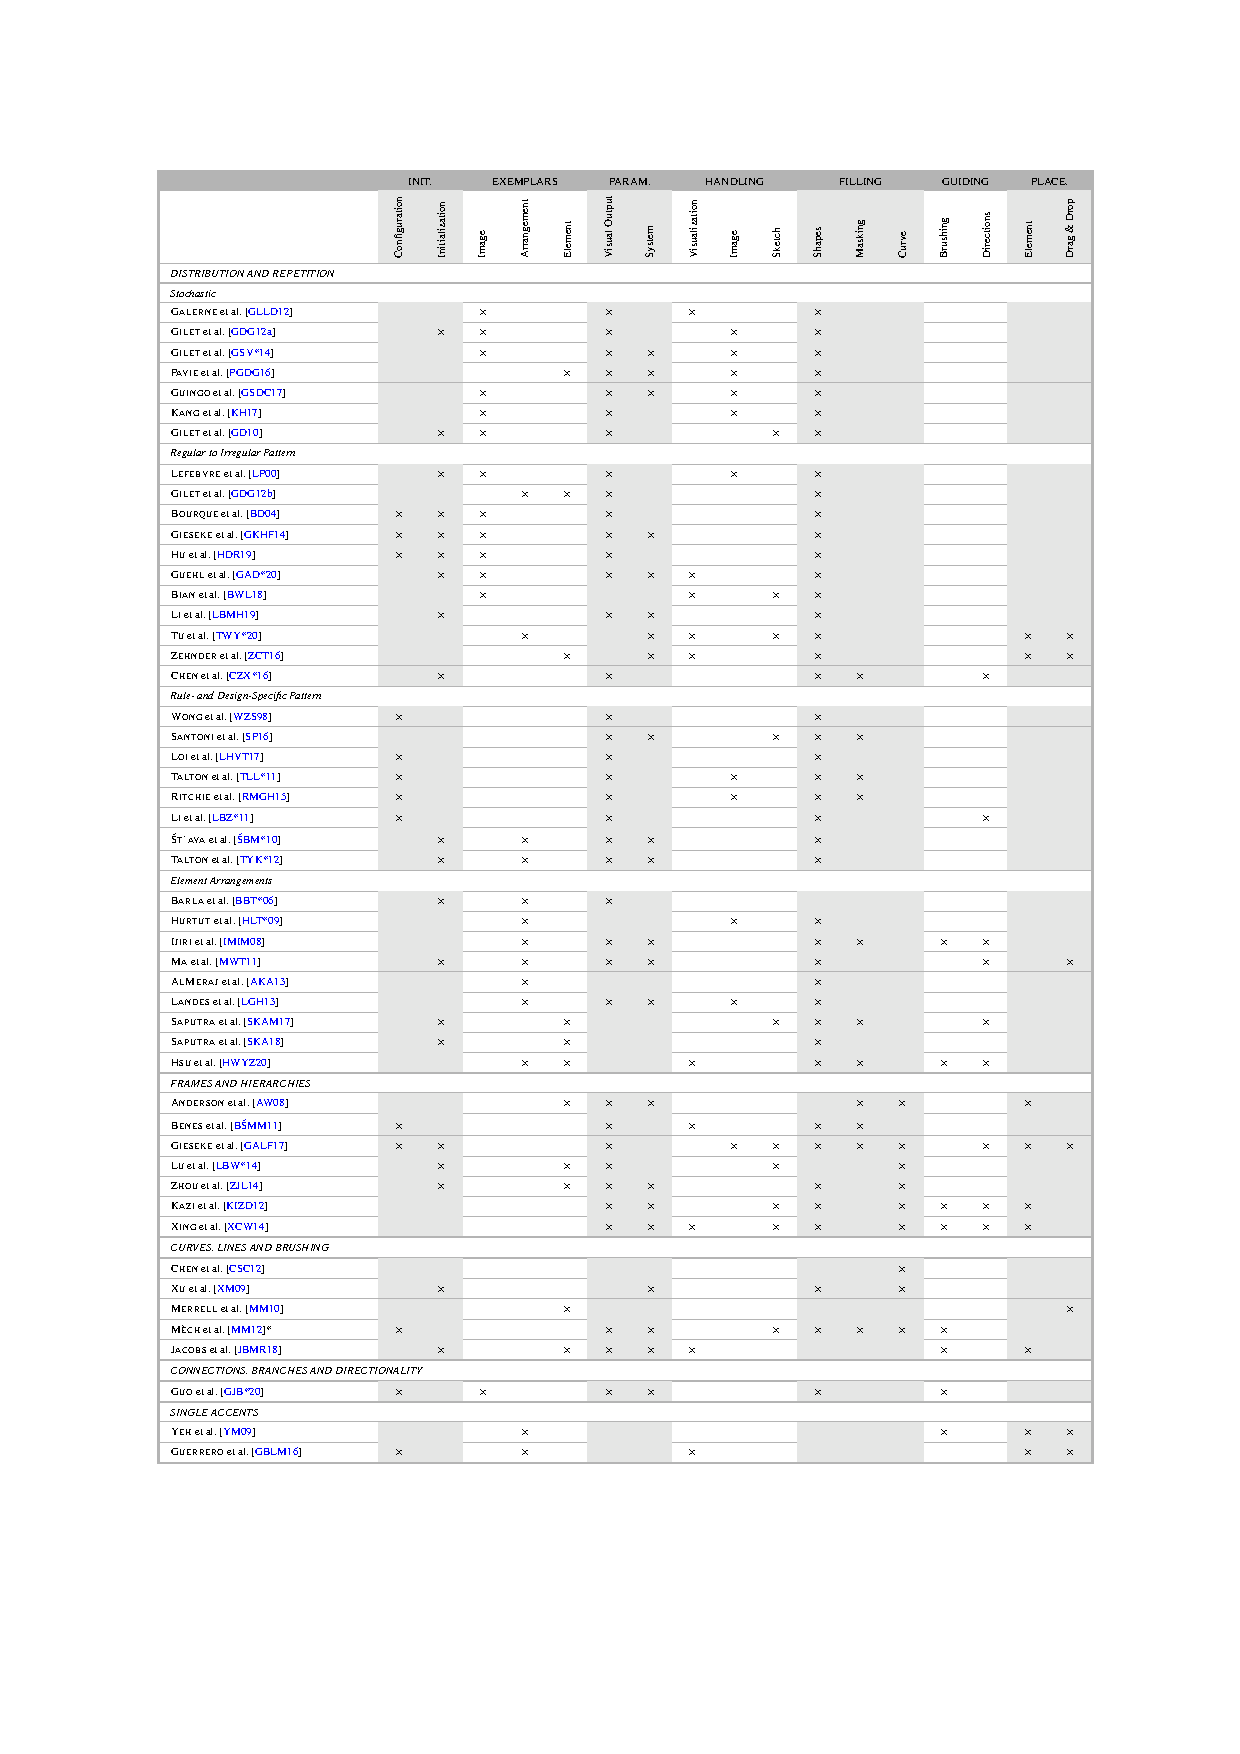
\includegraphics[width=0.85\textwidth]{tables/table_all.pdf}
    \caption[Control mechanisms in the state of the art]{Recent techniques are sorted by design areas and visual features they enable. For each work it is analysed and indicated which specific control mechanisms they offer. *Please note that \cite{mech_2012_tdf} present a procedural modeling engine, which in principle can be programmed to include almost any control type.\label{table:analysis}}
\end{table*}

